\section{Introduction}
\subsection{Case Overview}
This forensic investigation aims to examine a laptop that has been flagged on security systems as a result of unusual internet traffic. Using a \textbf{pcap} file, and \textbf{Okteta}, a Linux hex editor, I will investigate the user's network traffic to establish the cause of the suspicious traffic, and what files this user accessed and downloaded.

\subsection{Scope}
This investigation will be split into eight distinct sections.
\begin{itemize}
    \item Examine \textbf{anz-logo.jpg} and \textbf{bank-card.jpg}.
    \item Examine \textbf{ANZ1.jpg} and \textbf{ANZ2.jpg}.
    \item Examine \textbf{how-to-commit-crimes.docx}.
    \item Examine \textbf{ANZ\_Document.pdf, ANZ\_Document2.pdf,} and \textbf{evil.pdf}.
    \item Examine the Contents Within \textbf{hiddenmessage2.txt}.
    \item Examine \textbf{atm-image.jpg}.
    \item Examine \textbf{broken.jpg}.
    \item Examine \textbf{securepdf.pdf}.
\end{itemize}

\section{Section 1: Examine \textbf{anz-logo.jpg} and \textbf{bank-card.jpg}.}
\subsection{Tools Used}
\begin{itemize}
    \item \textbf{Wireshark}: a tool that sniffs web traffic for analysis
\end{itemize}

I started this investigation by opening my Wireshark to analyse the provided \textbf{pcap} file.

\begin{figure}[H]
    \setlength{\abovecaptionskip}{20pt}
    \setlength{\belowcaptionskip}{0pt}
    \centering
    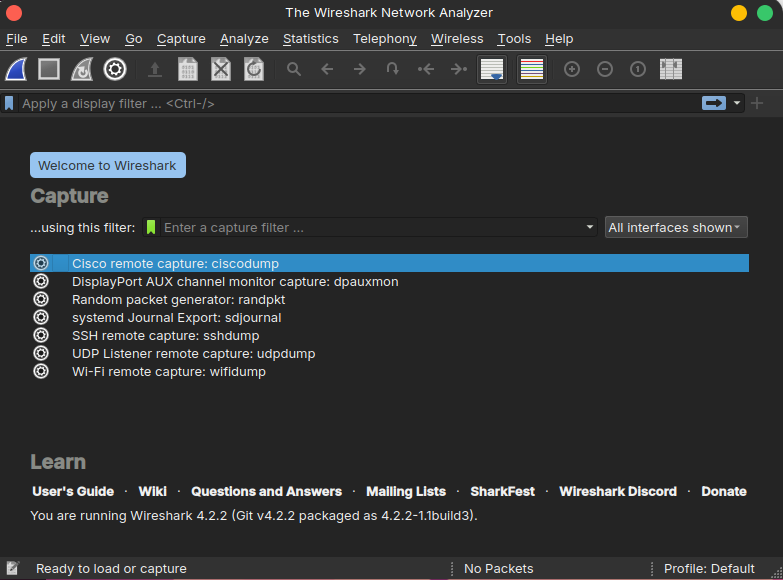
\includegraphics[width=0.7\textwidth]{1.png}
    \captionsetup{justification=centering}
    \caption{\textit{Wireshark UI.}}
    \label{fig:1}
\end{figure}
\vspace{-10pt}

From this, I opened the \textbf{pcap} file from the file manager.

\begin{figure}[H]
    \setlength{\abovecaptionskip}{20pt}
    \setlength{\belowcaptionskip}{0pt}
    \centering
    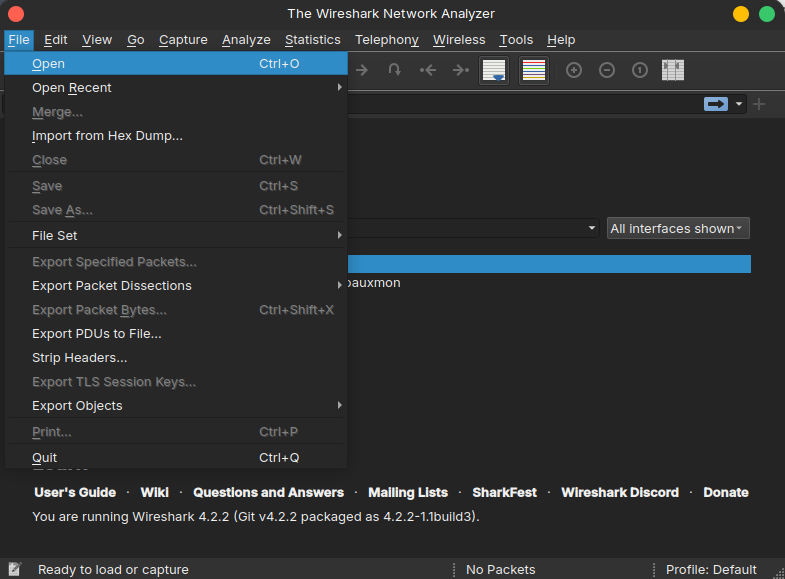
\includegraphics[width=0.7\textwidth]{2.png}
    \captionsetup{justification=centering}
    \caption{\textit{Opening File.}}
    \label{fig:2}
\end{figure}
\vspace{-10pt}

Navigating to \texttt{/home/b1ondie/Downloads}, I selected the file.

\begin{figure}[H]
    \setlength{\abovecaptionskip}{20pt}
    \setlength{\belowcaptionskip}{0pt}
    \centering
    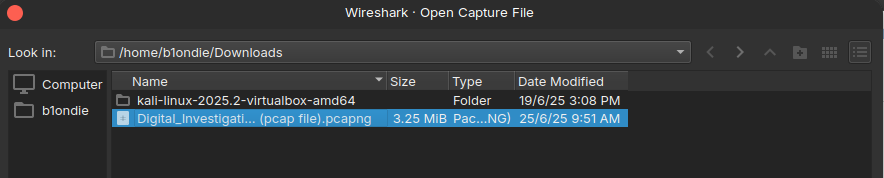
\includegraphics[width=0.8\textwidth]{3.png}
    \captionsetup{justification=centering}
    \caption{\textit{Selecting Given File.}}
    \label{fig:3}
\end{figure}
\vspace{-10pt}

Within the \textbf{pcap} file, I was able to view the network traffic generated by the user.

\begin{figure}[H]
    \setlength{\abovecaptionskip}{20pt}
    \setlength{\belowcaptionskip}{0pt}
    \centering
    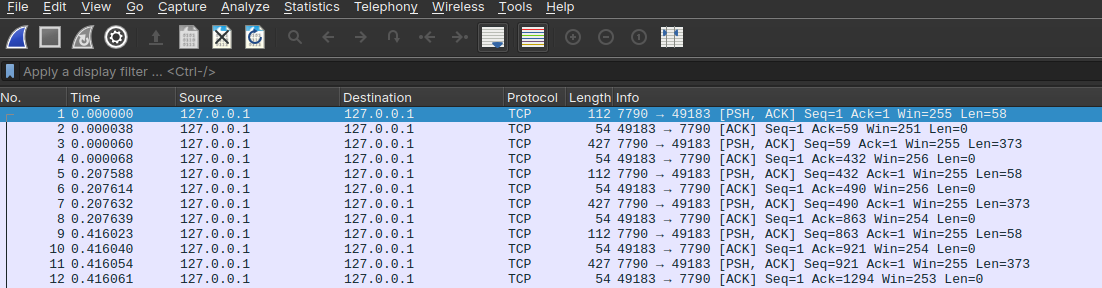
\includegraphics[width=1.0\textwidth]{5.png}
    \captionsetup{justification=centering}
    \caption{\textit{Viewing \textbf{pcap} File.}}
    \label{fig:5}
\end{figure}
\vspace{-10pt}

As per the request, I filtered the traffic to \textbf{http} to ensure I could analyse only HTTP traffic.

\begin{figure}[H]
    \setlength{\abovecaptionskip}{20pt}
    \setlength{\belowcaptionskip}{0pt}
    \centering
    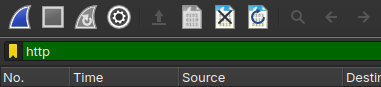
\includegraphics[width=0.5\textwidth]{6.png}
    \captionsetup{justification=centering}
    \caption{\textit{Filtering Traffic as HTTP.}}
    \label{fig:6}
\end{figure}
\vspace{-10pt}

I am now able to see all of the HTTP traffic generated by the user.

\begin{figure}[H]
    \setlength{\abovecaptionskip}{20pt}
    \setlength{\belowcaptionskip}{0pt}
    \centering
    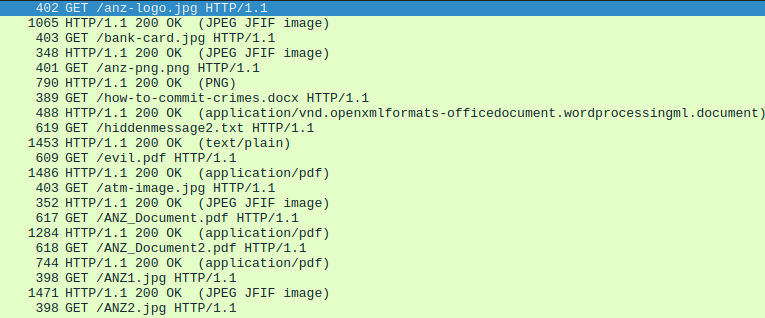
\includegraphics[width=0.8\textwidth]{7.png}
    \captionsetup{justification=centering}
    \caption{\textit{Analysing First Image.}}
    \label{fig:7}
\end{figure}
\vspace{-10pt}

In the first HTTP frame, I can see the user requested the \textbf{anz-logo.jpg} resource. 

\begin{figure}[H]
    \setlength{\abovecaptionskip}{20pt}
    \setlength{\belowcaptionskip}{0pt}
    \centering
    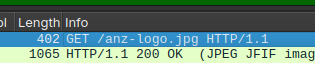
\includegraphics[width=0.4\textwidth]{8.png}
    \captionsetup{justification=centering}
    \caption{\textit{GET Request from Client.}}
    \label{fig:8}
\end{figure}
\vspace{-10pt}

Inspecting this packet, I can see that the server response is within frame \textbf{140}. 

\begin{figure}[H]
    \setlength{\abovecaptionskip}{20pt}
    \setlength{\belowcaptionskip}{0pt}
    \centering
    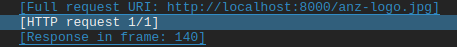
\includegraphics[width=0.6\textwidth]{9.png}
    \captionsetup{justification=centering}
    \caption{\textit{Response Note.}}
    \label{fig:9}
\end{figure}
\vspace{-10pt}

I navigate to this frame, and inspect its contents.

\begin{figure}[H]
    \setlength{\abovecaptionskip}{20pt}
    \setlength{\belowcaptionskip}{0pt}
    \centering
    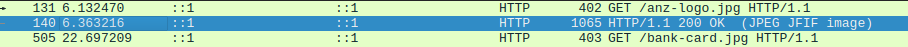
\includegraphics[width=1.0\textwidth]{10.png}
    \captionsetup{justification=centering}
    \caption{\textit{Response Frame from Server.}}
    \label{fig:10}
\end{figure}
\vspace{-10pt}

After doing some quick research\cite{sig}, I found the appropriate file signature for a \textbf{.jpg} file, which is \textbf{FF D8 FF E0}.

\begin{figure}[H]
    \setlength{\abovecaptionskip}{20pt}
    \setlength{\belowcaptionskip}{0pt}
    \centering
    
\includegraphics[width=1.0\textwidth]{11.png}
    \captionsetup{justification=centering}
    \caption{\textit{JPEG File Header\cite{sig}.}}
    \label{fig:11}
\end{figure}
\vspace{-10pt}

Inspecting the frame, I was able to find the \textbf{JPEG} file.

\begin{figure}[H]
    \setlength{\abovecaptionskip}{20pt}
    \setlength{\belowcaptionskip}{0pt}
    \centering
    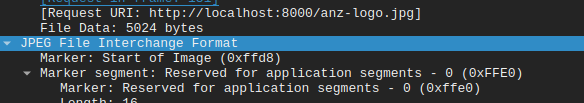
\includegraphics[width=0.7\textwidth]{12.png}
    \captionsetup{justification=centering}
    \caption{\textit{Packet Details.}}
    \label{fig:12}
\end{figure}
\vspace{-10pt}

I validated its file type by inspecting the raw bytes, which matched the file signature in my research. 

\begin{figure}[H]
    \setlength{\abovecaptionskip}{20pt}
    \setlength{\belowcaptionskip}{0pt}
    \centering
    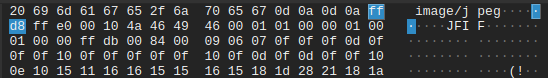
\includegraphics[width=0.7\textwidth]{13.png}
    \captionsetup{justification=centering}
    \caption{\textit{Packet Hex and ASCII Values.}}
    \label{fig:13}
\end{figure}
\vspace{-10pt}

I inspected the image itself, by right-clicking the \textbf{JPEG Filee Interchange Format} line, and clicking on \textbf{Show Packet Bytes}.

\begin{figure}[H]
    \setlength{\abovecaptionskip}{20pt}
    \setlength{\belowcaptionskip}{0pt}
    \centering
    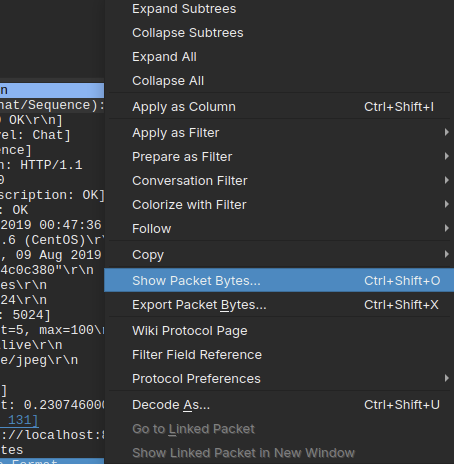
\includegraphics[width=0.5\textwidth]{14.png}
    \captionsetup{justification=centering}
    \caption{\textit{Show Packet Bytes Option.}}
    \label{fig:14}
\end{figure}
\vspace{-10pt}

I can now confirm that this is, in fact, an image file.

\begin{figure}[H]
    \setlength{\abovecaptionskip}{20pt}
    \setlength{\belowcaptionskip}{0pt}
    \centering
    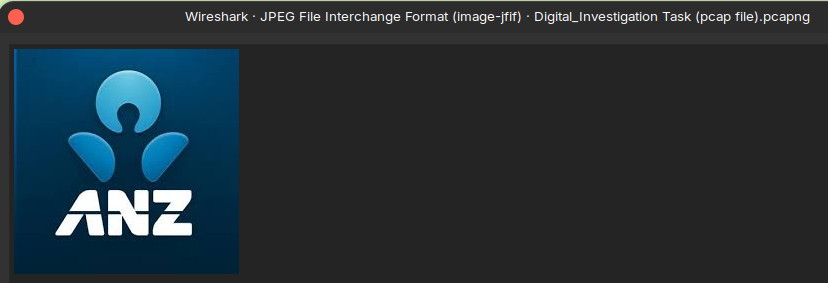
\includegraphics[width=0.8\textwidth]{15.png}
    \captionsetup{justification=centering}
    \caption{\textit{ANZ Image in Wireshark.}}
    \label{fig:15}
\end{figure}
\vspace{-10pt}

I proceed to export the image file, by right-clicking the same line, and selecting \textbf{Export Packet Bytes}.

\begin{figure}[H]
    \setlength{\abovecaptionskip}{20pt}
    \setlength{\belowcaptionskip}{0pt}
    \centering
    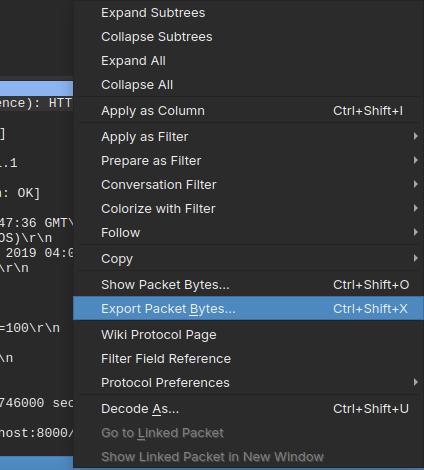
\includegraphics[width=0.5\textwidth]{16.png}
    \captionsetup{justification=centering}
    \caption{\textit{Export Packet Bytes Option.}}
    \label{fig:16}
\end{figure}
\vspace{-10pt}

I saved this on my local machine under \textbf{anz-logo.jpg}.

\begin{figure}[H]
    \setlength{\abovecaptionskip}{20pt}
    \setlength{\belowcaptionskip}{0pt}
    \centering
    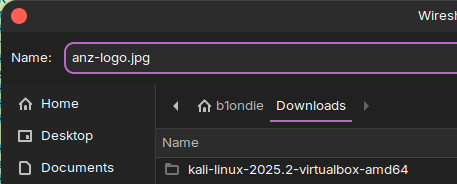
\includegraphics[width=0.5\textwidth]{17.png}
    \captionsetup{justification=centering}
    \caption{\textit{Saving Logo to File System.}}
    \label{fig:17}
\end{figure}
\vspace{-10pt}

I can now view this in my file system.

\begin{figure}[H]
    \setlength{\abovecaptionskip}{20pt}
    \setlength{\belowcaptionskip}{0pt}
    \centering
    
\includegraphics[width=0.2\textwidth]{18.png}
    \captionsetup{justification=centering}
    \caption{\textit{File Saved.}}
    \label{fig:18}
\end{figure}
\vspace{-10pt}

Opening the file heeds no errors, indicating that file extraction was a success.

\begin{figure}[H]
    \setlength{\abovecaptionskip}{20pt}
    \setlength{\belowcaptionskip}{0pt}
    \centering
    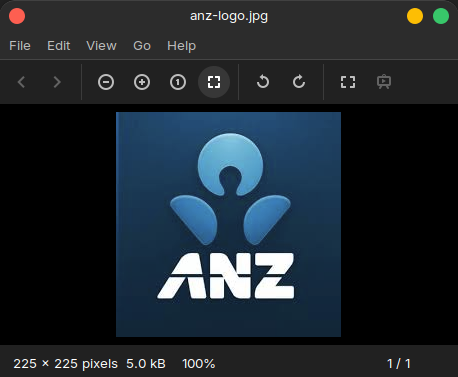
\includegraphics[width=0.5\textwidth]{19.png}
    \captionsetup{justification=centering}
    \caption{\textit{File Operable.}}
    \label{fig:19}
\end{figure}
\vspace{-10pt}

The full image contains the ANZ logo, in blue and white.

\begin{figure}[H]
    \setlength{\abovecaptionskip}{20pt}
    \setlength{\belowcaptionskip}{0pt}
    \centering
    
\includegraphics[width=0.3\textwidth]{20.jpg}
    \captionsetup{justification=centering}
    \caption{\textit{Full Image.}}
    \label{fig:20}
\end{figure}
\vspace{-10pt}

Inspecting the next file, \textbf{bank-card.jpg}, I followed the same procedure.

\begin{figure}[H]
    \setlength{\abovecaptionskip}{20pt}
    \setlength{\belowcaptionskip}{0pt}
    \centering
    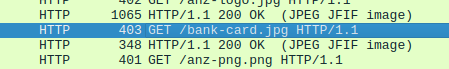
\includegraphics[width=0.6\textwidth]{21.png}
    \captionsetup{justification=centering}
    \caption{\textit{Second Image GET Request.}}
    \label{fig:21}
\end{figure}
\vspace{-10pt}

When the user has requested the image resource, the response from the server is provided in \textbf{frame 567}.

\begin{figure}[H]
    \setlength{\abovecaptionskip}{20pt}
    \setlength{\belowcaptionskip}{0pt}
    \centering
    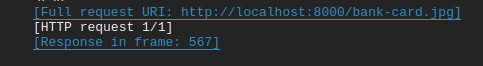
\includegraphics[width=0.6\textwidth]{22.png}
    \captionsetup{justification=centering}
    \caption{\textit{Response Note.}}
    \label{fig:22}
\end{figure}
\vspace{-10pt}

I proceed to navigate to this frame is Wireshark.

\begin{figure}[H]
    \setlength{\abovecaptionskip}{20pt}
    \setlength{\belowcaptionskip}{0pt}
    \centering
    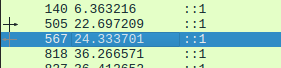
\includegraphics[width=0.4\textwidth]{23.png}
    \captionsetup{justification=centering}
    \caption{\textit{Response Packet.}}
    \label{fig:23}
\end{figure}
\vspace{-10pt}

Using the same method, I find the \textbf{JPEG File Interchange Format} line.

\begin{figure}[H]
    \setlength{\abovecaptionskip}{20pt}
    \setlength{\belowcaptionskip}{0pt}
    \centering
    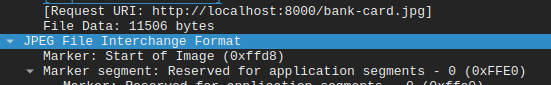
\includegraphics[width=0.7\textwidth]{24.png}
    \captionsetup{justification=centering}
    \caption{\textit{Packet Details.}}
    \label{fig:24}
\end{figure}
\vspace{-10pt}

Right-clicking this, I select \textbf{Export Packet Bytes}.

\begin{figure}[H]
    \setlength{\abovecaptionskip}{20pt}
    \setlength{\belowcaptionskip}{0pt}
    \centering
    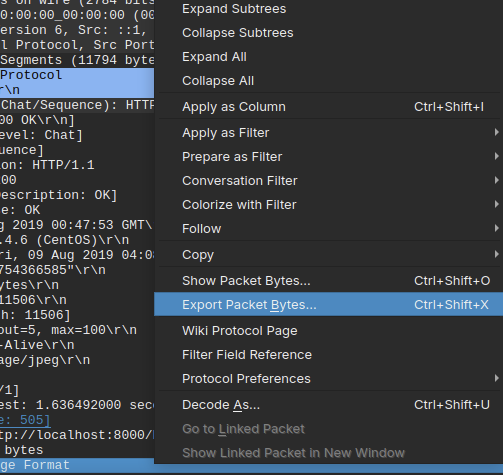
\includegraphics[width=0.5\textwidth]{25.png}
    \captionsetup{justification=centering}
    \caption{\textit{Export Packet Details Option.}}
    \label{fig:25}
\end{figure}
\vspace{-10pt}

This image is saved in my local file system under the name \textbf{bank-card.jpg}.

\begin{figure}[H]
    \setlength{\abovecaptionskip}{20pt}
    \setlength{\belowcaptionskip}{0pt}
    \centering
    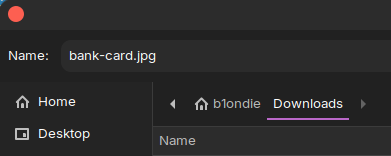
\includegraphics[width=0.5\textwidth]{26.png}
    \captionsetup{justification=centering}
    \caption{\textit{Saving File.}}
    \label{fig:26}
\end{figure}
\vspace{-10pt}

I can now view this in my file system.

\begin{figure}[H]
    \setlength{\abovecaptionskip}{20pt}
    \setlength{\belowcaptionskip}{0pt}
    \centering
    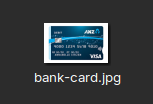
\includegraphics[width=0.2\textwidth]{27.png}
    \captionsetup{justification=centering}
    \caption{\textit{File Saved to File System.}}
    \label{fig:27}
\end{figure}
\vspace{-10pt}

I validate its integrity by opening the file. I can see the entire file in my image viewer, which demonstrates file extraction was a success.

\begin{figure}[H]
    \setlength{\abovecaptionskip}{20pt}
    \setlength{\belowcaptionskip}{0pt}
    \centering
    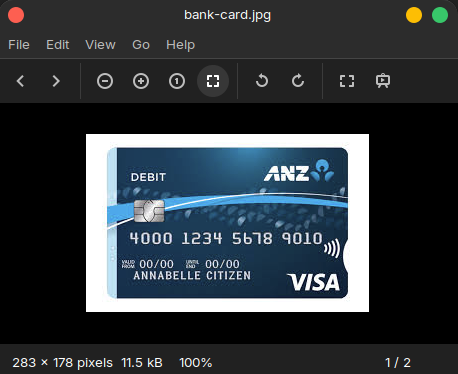
\includegraphics[width=0.5\textwidth]{28.png}
    \captionsetup{justification=centering}
    \caption{\textit{File Operable.}}
    \label{fig:28}
\end{figure}
\vspace{-10pt}

The full image appears to be a bank card, addresses to an \textbf{Annabelle Citizen}, with the full card number shown, \textbf{4000 1234 5678 9010}. 

\begin{figure}[H]
    \setlength{\abovecaptionskip}{20pt}
    \setlength{\belowcaptionskip}{0pt}
    \centering
    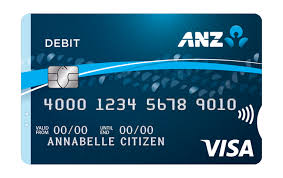
\includegraphics[width=0.4\textwidth]{29.jpg}
    \captionsetup{justification=centering}
    \caption{\textit{Full Image.}}
    \label{fig:29}
\end{figure}
\vspace{-10pt}

\section{Section 2: Examine \textbf{ANZ1.jpg} and \textbf{ANZ2.jpg}.}
\subsection{Tools Used}
\begin{itemize}
    \item \textbf{Wireshark}
\end{itemize}

I first examined a regular image that the server had sent to the user.

\begin{figure}[H]
    \setlength{\abovecaptionskip}{20pt}
    \setlength{\belowcaptionskip}{0pt}
    \centering
    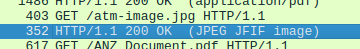
\includegraphics[width=0.5\textwidth]{38.png}
    \captionsetup{justification=centering}
    \caption{\textit{Image GET Request.}}
    \label{fig:38}
\end{figure}
\vspace{-10pt}

Upon examining this file, I analysed the file structure as a means of comparison to \textbf{ANZ1.jpg}, and \textbf{ANZ2.jpg}.

\begin{figure}[H]
    \setlength{\abovecaptionskip}{20pt}
    \setlength{\belowcaptionskip}{0pt}
    \centering
    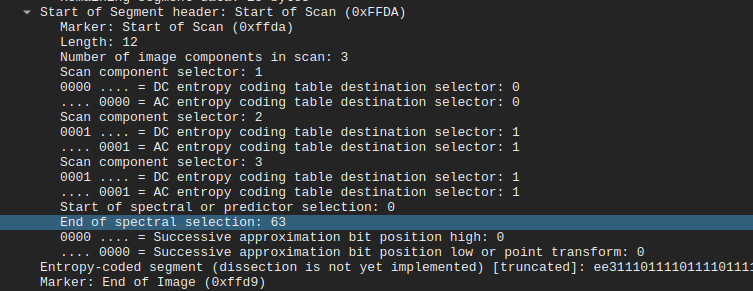
\includegraphics[width=0.7\textwidth]{39.png}
    \captionsetup{justification=centering}
    \caption{\textit{Packet Details.}}
    \label{fig:39}
\end{figure}
\vspace{-10pt}

I then navigated to \textbf{ANZ1.jpg}.

\begin{figure}[H]
    \setlength{\abovecaptionskip}{20pt}
    \setlength{\belowcaptionskip}{0pt}
    \centering
    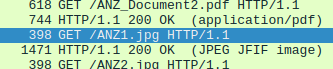
\includegraphics[width=0.4\textwidth]{40.png}
    \captionsetup{justification=centering}
    \caption{\textit{Image GET Request.}}
    \label{fig:40}
\end{figure}
\vspace{-10pt}

Within this image, I noticed an additional line at the bottom of the frame data, denoted \textbf{Entropy-coded segment (dissection is not yet implemented): 596f7527766520666f756e6420612068696464656e206d65737361676520\\
696e20746869732066696c652120496e636c75646520697420696e20796f75722077726974652075702e0a}. 

\begin{figure}[H]
    \setlength{\abovecaptionskip}{20pt}
    \setlength{\belowcaptionskip}{0pt}
    \centering
    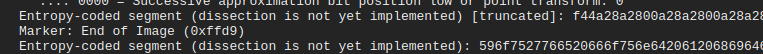
\includegraphics[width=0.8\textwidth]{41.png}
    \captionsetup{justification=centering}
    \caption{\textit{Hidden String in Packet.}}
    \label{fig:41}
\end{figure}
\vspace{-10pt}

When analysing the data further, a secret message appears in the \textbf{ASCII} panel of Wireshark:\\
\texttt{You've found a hidden message in this file! Include it in your write up.}

\begin{figure}[H]
    \setlength{\abovecaptionskip}{20pt}
    \setlength{\belowcaptionskip}{0pt}
    \centering
    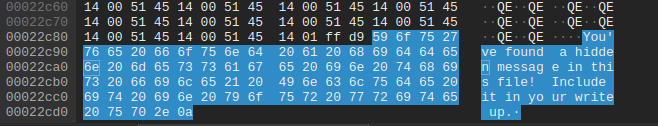
\includegraphics[width=0.7\textwidth]{42.png}
    \captionsetup{justification=centering}
    \caption{\textit{Hidden String in ASCII Panel.}}
    \label{fig:42}
\end{figure}
\vspace{-10pt}

I noticed \textbf{ANZ2.jpg} also contained a similar file structure.

\begin{figure}[H]
    \setlength{\abovecaptionskip}{20pt}
    \setlength{\belowcaptionskip}{0pt}
    \centering
    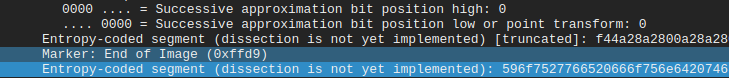
\includegraphics[width=0.8\textwidth]{43.png}
    \captionsetup{justification=centering}
    \caption{\textit{ANZ2.jpg Presents Same File Structure.}}
    \label{fig:43}
\end{figure}
\vspace{-10pt}

Scrolling to the last bytes of the file, I notice a similar hidden message to the one above, which reads:\\
\texttt{You've found a hidden message! Images are sometimes more than they appear.}

\begin{figure}[H]
    \setlength{\abovecaptionskip}{20pt}
    \setlength{\belowcaptionskip}{0pt}
    \centering
    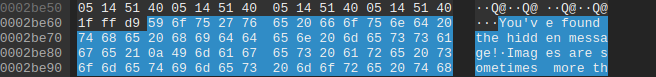
\includegraphics[width=0.7\textwidth]{44.png}
    \captionsetup{justification=centering}
    \caption{\textit{Hidden String in ASCII Panel.}}
    \label{fig:44}
\end{figure}
\vspace{-10pt}

To extract the files, I right-clicked the image file in the frame and selected the \textbf{Export Packet Bytes} option as usual.

\begin{figure}[H]
    \setlength{\abovecaptionskip}{20pt}
    \setlength{\belowcaptionskip}{0pt}
    \centering
    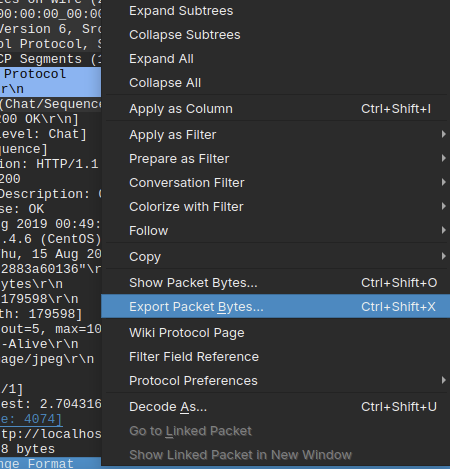
\includegraphics[width=0.5\textwidth]{45.png}
    \captionsetup{justification=centering}
    \caption{\textit{Export Packet Bytes Option.}}
    \label{fig:45}
\end{figure}
\vspace{-10pt}

I can now see these images in my file system.

\begin{figure}[H]
    \setlength{\abovecaptionskip}{20pt}
    \setlength{\belowcaptionskip}{0pt}
    \centering
    
\includegraphics[width=0.3\textwidth]{46.png}
    \captionsetup{justification=centering}
    \caption{\textit{Two Images in File System.}}
    \label{fig:46}
\end{figure}
\vspace{-10pt}

Opening the files validates their integrity, as they have not been corruputed in the extraction process, and work as expected.

\begin{figure}[H]
    \setlength{\abovecaptionskip}{20pt}
    \setlength{\belowcaptionskip}{0pt}
    \centering
    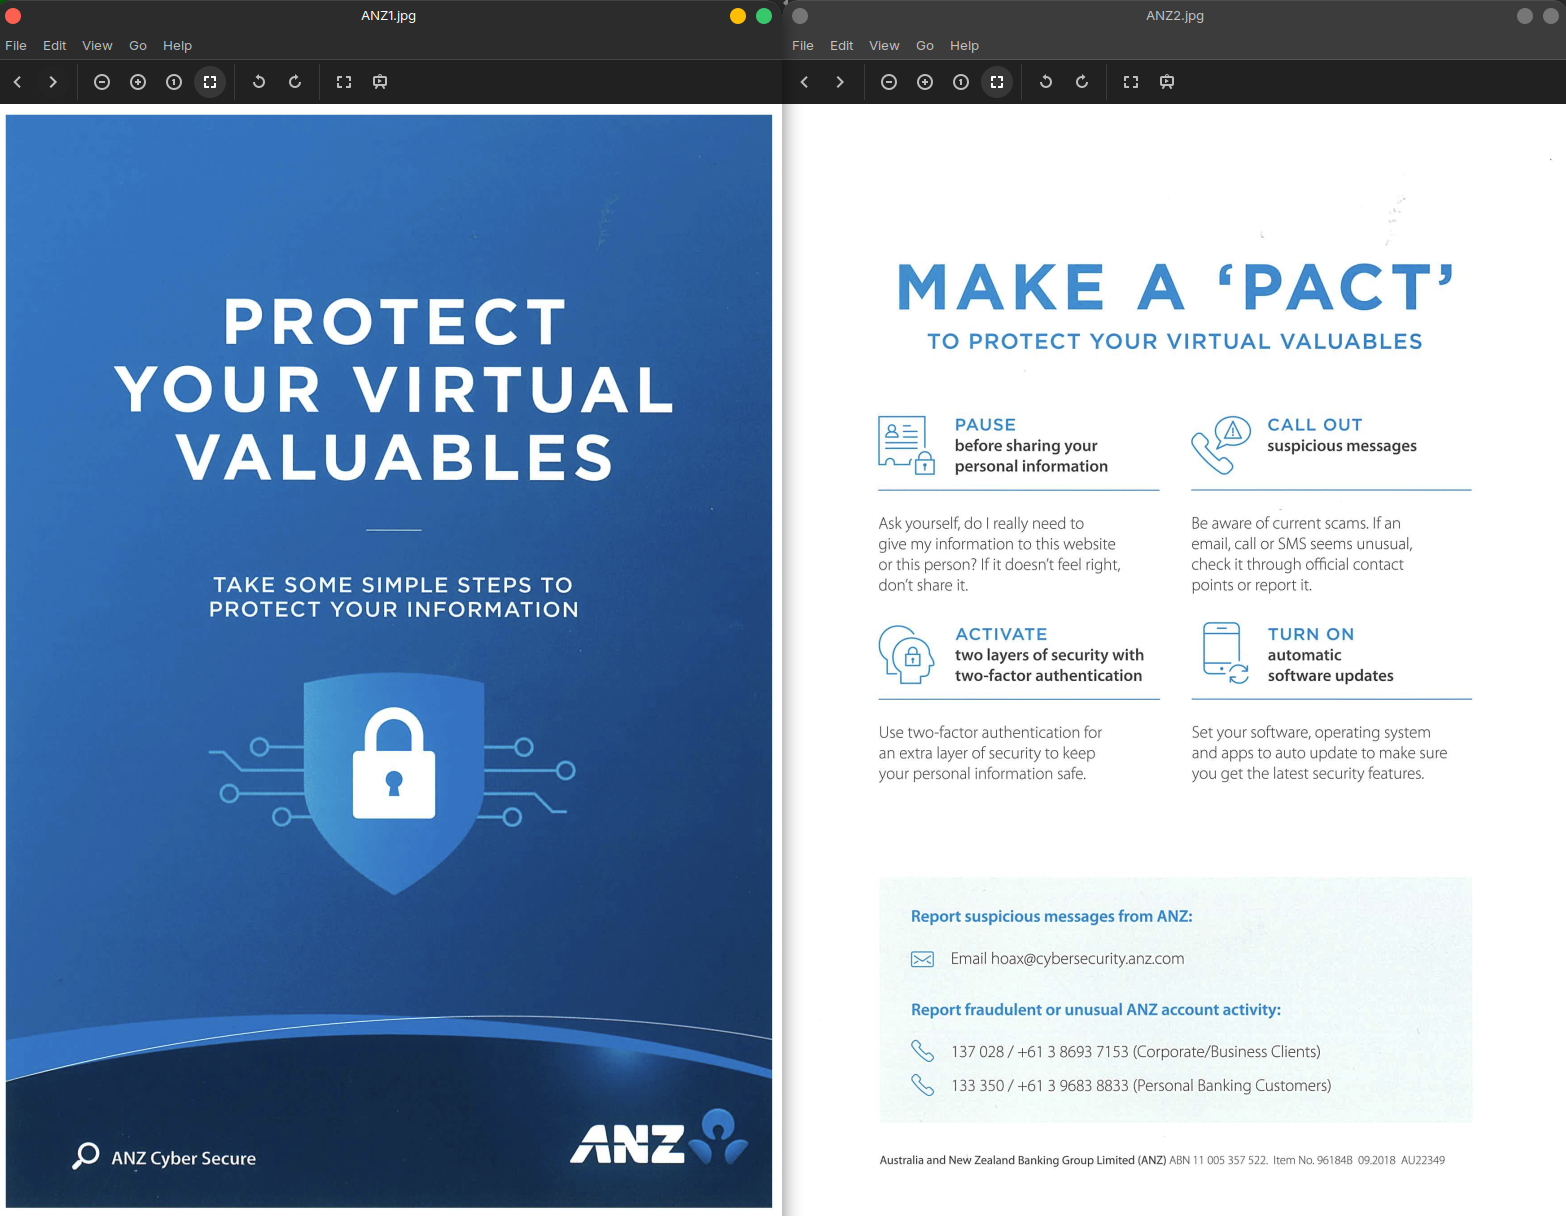
\includegraphics[width=0.7\textwidth]{47.png}
    \captionsetup{justification=centering}
    \caption{\textit{Extracted JPG's.}}
    \label{fig:47}
\end{figure}
\vspace{-10pt}

\textbf{ANZ1.jpg} is an awareness poster made by ANZ prompting the viewer to \textbf{protect [their] virtual valuables}.

\begin{figure}[H]
    \setlength{\abovecaptionskip}{20pt}
    \setlength{\belowcaptionskip}{0pt}
    \centering
    
\includegraphics[width=0.6\textwidth]{48.png}
    \captionsetup{justification=centering}
    \caption{\textit{First JPG.}}
    \label{fig:48}
\end{figure}
\vspace{-10pt}

\textbf{ANZ2.jpg} is another awareness poster on \textit{how} one can protect their virtual valuables.

\begin{figure}[H]
    \setlength{\abovecaptionskip}{20pt}
    \setlength{\belowcaptionskip}{0pt}
    \centering
    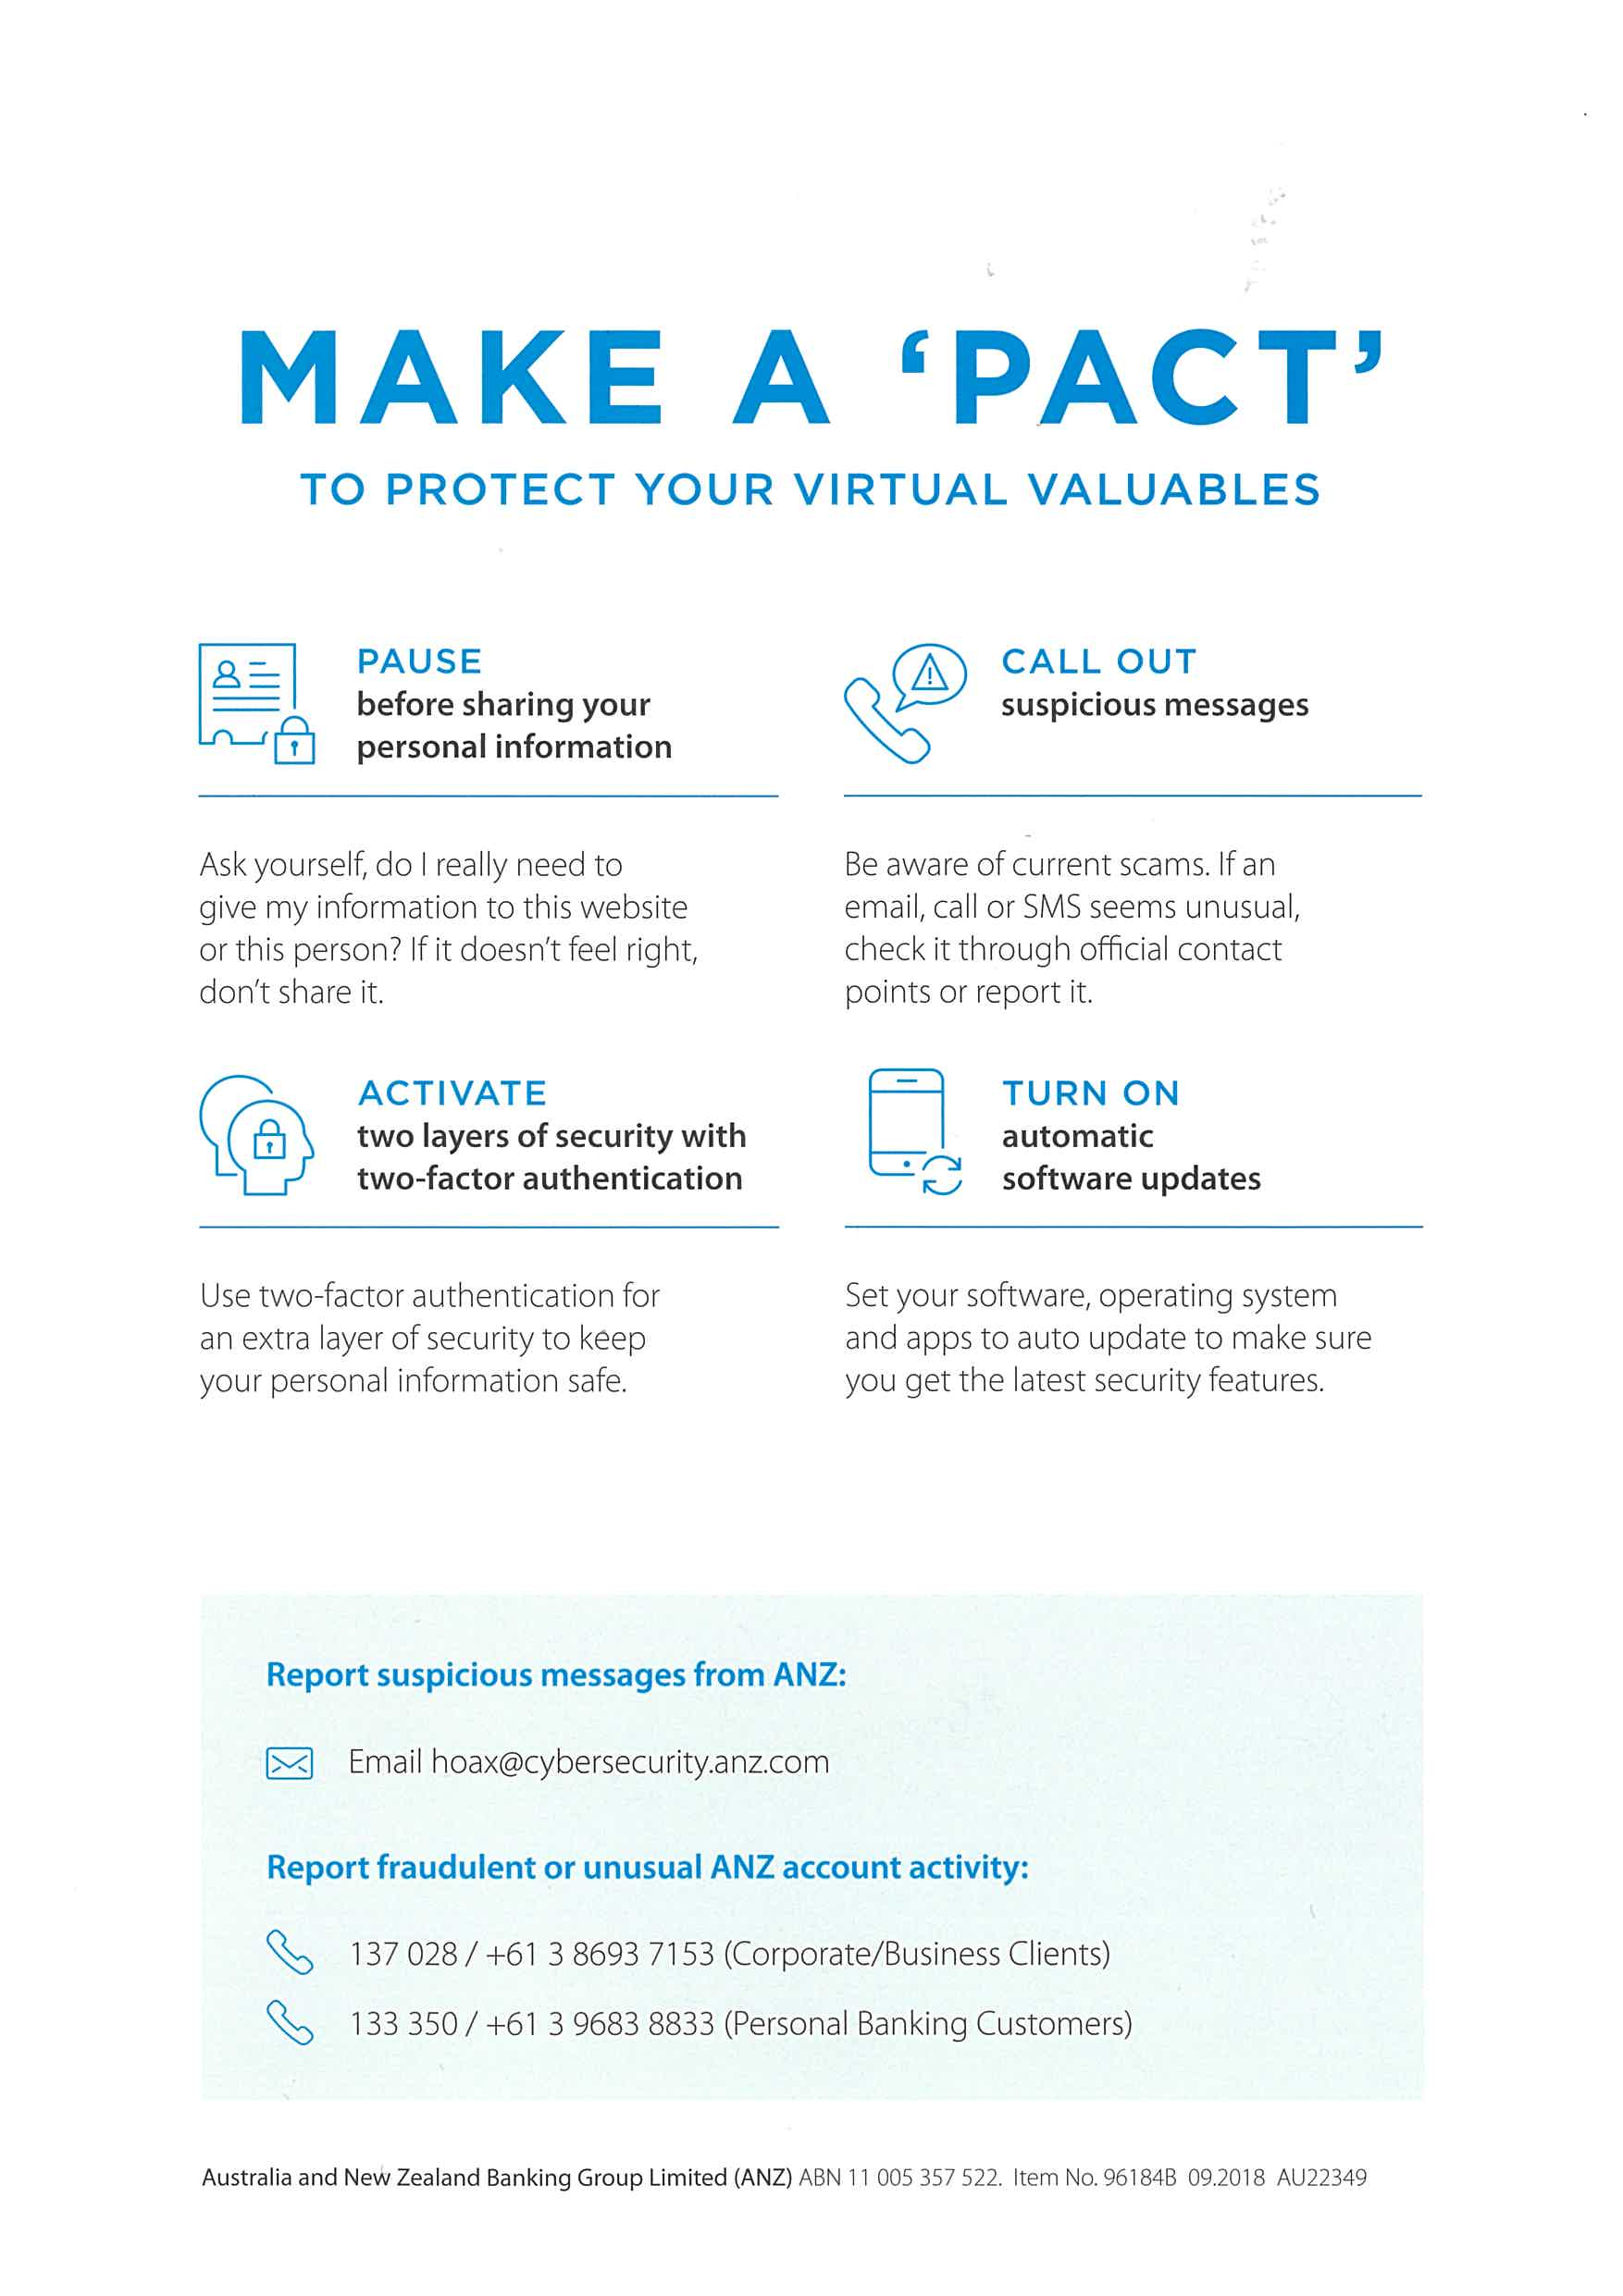
\includegraphics[width=0.6\textwidth]{49.png}
    \captionsetup{justification=centering}
    \caption{\textit{Second JPG.}}
    \label{fig:49}
\end{figure}
\vspace{-10pt}

\section{Section 3: Examine \textbf{how-to-commit-crimes.docx}.}
\subsection{Tools Used}
\begin{itemize}
    \item \textbf{Wireshark}
\end{itemize}

I searched through the packets in Wireshark until I found \textbf{how-to-commit-crimes.docx}. 

\begin{figure}[H]
    \setlength{\abovecaptionskip}{20pt}
    \setlength{\belowcaptionskip}{0pt}
    \centering
    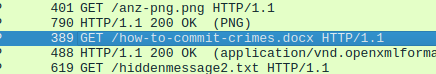
\includegraphics[width=0.5\textwidth]{30.png}
    \captionsetup{justification=centering}
    \caption{\textit{docx GET Request.}}
    \label{fig:30}
\end{figure}
\vspace{-10pt}

The very next frame displays the requested content provided by the server.

\begin{figure}[H]
    \setlength{\abovecaptionskip}{20pt}
    \setlength{\belowcaptionskip}{0pt}
    \centering
    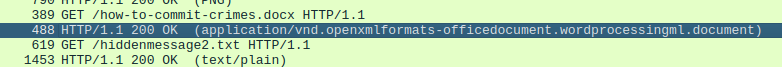
\includegraphics[width=0.9\textwidth]{31.png}
    \captionsetup{justification=centering}
    \caption{\textit{Response Packet from Server.}}
    \label{fig:31}
\end{figure}
\vspace{-10pt}

Within this frame, I notice that the document is an Word Processing XML document. 

\begin{figure}[H]
    \setlength{\abovecaptionskip}{20pt}
    \setlength{\belowcaptionskip}{0pt}
    \centering
    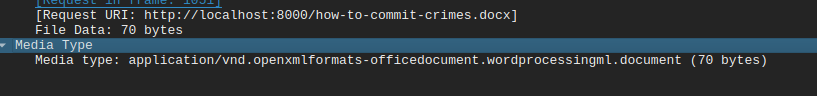
\includegraphics[width=0.8\textwidth]{32.png}
    \captionsetup{justification=centering}
    \caption{\textit{Media Type of Payload.}}
    \label{fig:32}
\end{figure}
\vspace{-10pt}

Analysing the contents of the document in the \textbf{ASCII/Raw Bytes panel} of Wireshark, I notice the following words:\\
\texttt{Step 1: Find target.}\\
\texttt{Step 2: Hack them.}\\
\texttt{This is a suspicious document.}\\

\begin{figure}[H]
    \setlength{\abovecaptionskip}{20pt}
    \setlength{\belowcaptionskip}{0pt}
    \centering
    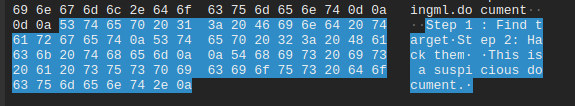
\includegraphics[width=0.7\textwidth]{33.png}
    \captionsetup{justification=centering}
    \caption{\textit{Suspicious Strings in docx.}}
    \label{fig:33}
\end{figure}
\vspace{-10pt}

To analyse the file further, I export the bytes using the option \textbf{Export Packet Bytes}.

\begin{figure}[H]
    \setlength{\abovecaptionskip}{20pt}
    \setlength{\belowcaptionskip}{0pt}
    \centering
    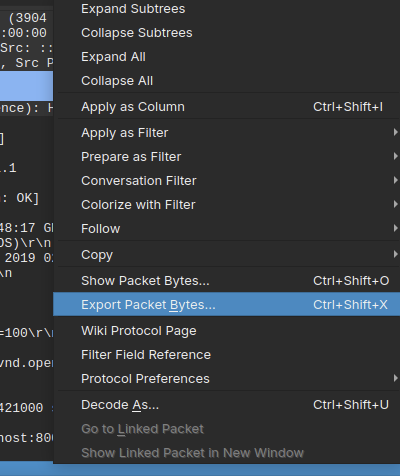
\includegraphics[width=0.5\textwidth]{34.png}
    \captionsetup{justification=centering}
    \caption{\textit{Export Packet Bytes Option.}}
    \label{fig:34}
\end{figure}
\vspace{-10pt}

A new window pops up and I input the file name \textbf{how-to-commit-crimes.docx} to maintain the integrity of the file type.

\begin{figure}[H]
    \setlength{\abovecaptionskip}{20pt}
    \setlength{\belowcaptionskip}{0pt}
    \centering
    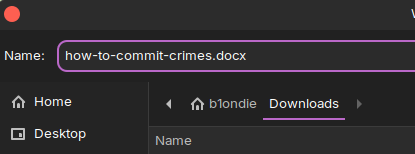
\includegraphics[width=0.5\textwidth]{35.png}
    \captionsetup{justification=centering}
    \caption{\textit{Extracting File.}}
    \label{fig:35}
\end{figure}
\vspace{-10pt}

This file is now available to view in my file system.

\begin{figure}[H]
    \setlength{\abovecaptionskip}{20pt}
    \setlength{\belowcaptionskip}{0pt}
    \centering
    
\includegraphics[width=0.2\textwidth]{36.png}
    \captionsetup{justification=centering}
    \caption{\textit{Extracted File in File System.}}
    \label{fig:36}
\end{figure}
\vspace{-10pt}

When opened with LibreOffice, I can now see the entirety of the file contents as I first discovered in Wireshark. This confirms that the file contents is indeed:\\
\texttt{Step 1: Find target.}\\
\texttt{Step 2: Hack them.}\\
\texttt{This is a suspicious document.}\\

\begin{figure}[H]
    \setlength{\abovecaptionskip}{20pt}
    \setlength{\belowcaptionskip}{0pt}
    \centering
    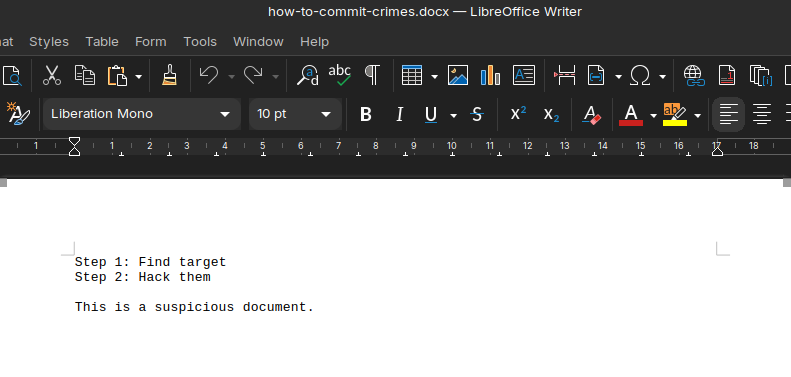
\includegraphics[width=0.8\textwidth]{37.png}
    \captionsetup{justification=centering}
    \caption{\textit{File is Operable and Displays Secret Message.}}
    \label{fig:37}
\end{figure}
\vspace{-10pt}

\section{Section 4: Examine \textbf{ANZ\_Document.pdf, ANZ\_Document2.pdf,} and \textbf{evil.pdf}.}
\subsection{Tools Used}
\begin{itemize}
    \item \textbf{Wireshark}
\end{itemize}

Tracing the clients resource request for \textbf{ANZ\_Document.pdf}, I was able to locate the server's response. 

\begin{figure}[H]
    \setlength{\abovecaptionskip}{20pt}
    \setlength{\belowcaptionskip}{0pt}
    \centering
    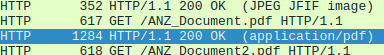
\includegraphics[width=0.5\textwidth]{50.png}
    \captionsetup{justification=centering}
    \caption{\textit{PDF GET Request.}}
    \label{fig:50}
\end{figure}
\vspace{-10pt}

As usual, I export the file using \textbf{Export Packet Bytes}.

\begin{figure}[H]
    \setlength{\abovecaptionskip}{20pt}
    \setlength{\belowcaptionskip}{0pt}
    \centering
    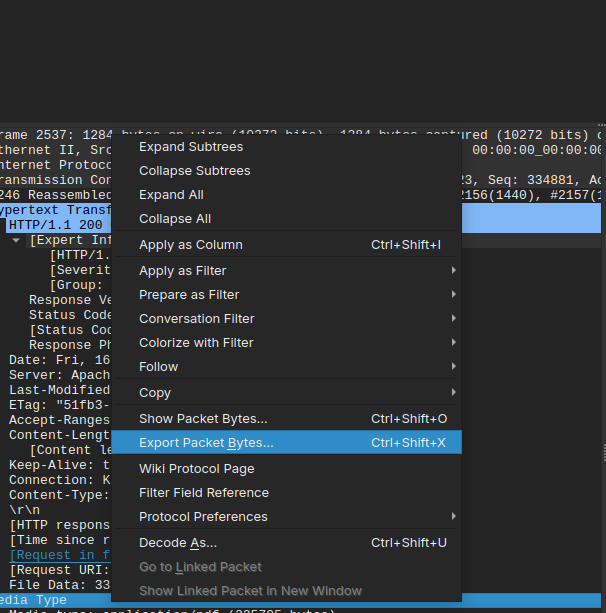
\includegraphics[width=0.6\textwidth]{51.png}
    \captionsetup{justification=centering}
    \caption{\textit{PDF GET Request.}}
    \label{fig:51}
\end{figure}
\vspace{-10pt}

I extract this file, naming it \textbf{ANZ\_Document.pdf}.

\begin{figure}[H]
    \setlength{\abovecaptionskip}{20pt}
    \setlength{\belowcaptionskip}{0pt}
    \centering
    \includegraphics[width=0.5\textwidth]{52.png}
    \captionsetup{justification=centering}
    \caption{\textit{Export Packet Bytes Option.}}
    \label{fig:52}
\end{figure}
\vspace{-10pt}

I follow the same process for \textbf{ANZ\_Document2}, where I am able to find the document in question.

\begin{figure}[H]
    \setlength{\abovecaptionskip}{20pt}
    \setlength{\belowcaptionskip}{0pt}
    \centering
    \includegraphics[width=0.5\textwidth]{53.png}
    \captionsetup{justification=centering}
    \caption{\textit{Extracting ANZ\_Document.pdf.}}
    \label{fig:53}
\end{figure}
\vspace{-10pt}

I extract this file as well using \textbf{Export Packet Bytes}.

\begin{figure}[H]
    \setlength{\abovecaptionskip}{20pt}
    \setlength{\belowcaptionskip}{0pt}
    \centering
    \includegraphics[width=0.6\textwidth]{54.png}
    \captionsetup{justification=centering}
    \caption{\textit{Export Packet Bytes Option}}
    \label{fig:54}
\end{figure}
\vspace{-10pt}

This is saved to my file system under \textbf{ANZ\_Document2.pdf}.

\begin{figure}[H]
    \setlength{\abovecaptionskip}{20pt}
    \setlength{\belowcaptionskip}{0pt}
    \centering
    \includegraphics[width=0.5\textwidth]{55.png}
    \captionsetup{justification=centering}
    \caption{\textit{Extracting PDF File.}}
    \label{fig:55}
\end{figure}
\vspace{-10pt}

I followed the same process to find the \textbf{evil.pdf} file in the HTTP traffic.

\begin{figure}[H]
    \setlength{\abovecaptionskip}{20pt}
    \setlength{\belowcaptionskip}{0pt}
    \centering
    \includegraphics[width=0.5\textwidth]{60.png}
    \captionsetup{justification=centering}
    \caption{\textit{PDF GET Request.}}
    \label{fig:60}
\end{figure}
\vspace{-10pt}

Opening the server packet, I exported the PDF using \textbf{Export Packet Bytes}.

\begin{figure}[H]
    \setlength{\abovecaptionskip}{20pt}
    \setlength{\belowcaptionskip}{0pt}
    \centering
    \includegraphics[width=0.7\textwidth]{61.png}
    \captionsetup{justification=centering}
    \caption{\textit{Export Packet Bytes Option.}}
    \label{fig:61}
\end{figure}
\vspace{-10pt}

This was subsequently saved as \textbf{evil.pdf} in my file system.

\begin{figure}[H]
    \setlength{\abovecaptionskip}{20pt}
    \setlength{\belowcaptionskip}{0pt}
    \centering
    \includegraphics[width=0.6\textwidth]{62.png}
    \captionsetup{justification=centering}
    \caption{\textit{Extracting File.}}
    \label{fig:62}
\end{figure}
\vspace{-10pt}

I am now able to view all three files in my file system. 

\begin{figure}[H]
    \setlength{\abovecaptionskip}{20pt}
    \setlength{\belowcaptionskip}{0pt}
    \centering
    \includegraphics[width=0.4\textwidth]{56.png}
    \captionsetup{justification=centering}
    \caption{\textit{All Files Extracted.}}
    \label{fig:56}
\end{figure}
\vspace{-10pt}

Opening the files demonstrates their integrity, as I receive no unexpected errors. 

\begin{figure}[H]
    \setlength{\abovecaptionskip}{20pt}
    \setlength{\belowcaptionskip}{0pt}
    \centering
    \includegraphics[width=0.8\textwidth]{57.png}
    \captionsetup{justification=centering}
    \caption{\textit{Files Available to View.}}
    \label{fig:57}
\end{figure}
\vspace{-10pt}

\begin{figure}[H]
    \setlength{\abovecaptionskip}{20pt}
    \setlength{\belowcaptionskip}{0pt}
    \centering
    \includegraphics[width=0.8\textwidth]{63.png}
    \captionsetup{justification=centering}
    \caption{\textit{Hidden Message in evil.pdf.}}
    \label{fig:63}
\end{figure}
\vspace{-10pt}

\textbf{ANZ\_Document.pdf} displays what seems to be the first page of a Cybersecurity document from ANZ. 

\begin{figure}[H]
    \setlength{\abovecaptionskip}{20pt}
    \setlength{\belowcaptionskip}{0pt}
    \centering
    \includegraphics[width=0.8\textwidth]{58.png}
    \captionsetup{justification=centering}
    \caption{\textit{Full PDF.}}
    \label{fig:58}
\end{figure}
\vspace{-10pt}

\textbf{ANZ\_Document2.pdf} appears to be another two pages from the same document, namely pages 3 and 4.

\begin{figure}[H]
    \setlength{\abovecaptionskip}{20pt}
    \setlength{\belowcaptionskip}{0pt}
    \centering
    \includegraphics[width=0.8\textwidth]{59.png}
    \captionsetup{justification=centering}
    \caption{\textit{Full PDF.}}
    \label{fig:59}
\end{figure}
\vspace{-10pt}

\textbf{evil.pdf} contains two pages, the first of which is completely blue, and the second which has a hidden message: \texttt{More suspicious stuff good job!}.

\begin{figure}[H]
    \setlength{\abovecaptionskip}{20pt}
    \setlength{\belowcaptionskip}{0pt}
    \centering
    \includegraphics[width=0.5\textwidth]{64.png}
    \captionsetup{justification=centering}
    \caption{\textit{First Page of evil.pdf.}}
    \label{fig:64}
\end{figure}
\vspace{-10pt}

\begin{figure}[H]
    \setlength{\abovecaptionskip}{20pt}
    \setlength{\belowcaptionskip}{0pt}
    \centering
    \includegraphics[width=0.7\textwidth]{65.png}
    \captionsetup{justification=centering}
    \caption{\textit{Second Page of PDF.}}
    \label{fig:65}
\end{figure}
\vspace{-10pt}

\section{Section 5: Examine the Contents Within \textbf{hiddenmessage2.txt}.}
\subsection{Tools Used}
\begin{itemize}
    \item \textbf{Wireshark}
    \item \textbf{Linux Mint Text Editor}: a tool that can edit and modify text files
\end{itemize}

This part of the investigation explores analysing file signatures. To start, I navigated to the \textbf{hiddenmessage2.txt} file resource sent from the server.

\begin{figure}[H]
    \setlength{\abovecaptionskip}{20pt}
    \setlength{\belowcaptionskip}{0pt}
    \centering
    \includegraphics[width=0.5\textwidth]{66.png}
    \captionsetup{justification=centering}
    \caption{\textit{.txt GET Request.}}
    \label{fig:66}
\end{figure}
\vspace{-10pt}

From here, I extract the file using \textbf{Export Packet Bytes}. 

\begin{figure}[H]
    \setlength{\abovecaptionskip}{20pt}
    \setlength{\belowcaptionskip}{0pt}
    \centering
    \includegraphics[width=0.6\textwidth]{67.png}
    \captionsetup{justification=centering}
    \caption{\textit{Export Packet Bytes Option.}}
    \label{fig:67}
\end{figure}
\vspace{-10pt}

Before saving this to my file system under the name \textbf{hiddenmessage.txt}.

\begin{figure}[H]
    \setlength{\abovecaptionskip}{20pt}
    \setlength{\belowcaptionskip}{0pt}
    \centering
    \includegraphics[width=0.6\textwidth]{68.png}
    \captionsetup{justification=centering}
    \caption{\textit{Extracting .txt File.}}
    \label{fig:68}
\end{figure}
\vspace{-10pt}

Opening this file in my text editor, I noticed that the values looked very similar to what you would see in an image file.

\begin{figure}[H]
    \setlength{\abovecaptionskip}{20pt}
    \setlength{\belowcaptionskip}{0pt}
    \centering
    \includegraphics[width=1.0\textwidth]{69.png}
    \captionsetup{justification=centering}
    \caption{\textit{Viewing File in Text Editor.}}
    \label{fig:69}
\end{figure}
\vspace{-10pt}

Investigating further, I can see that the file is, in fact, an image file, specifically a JPEG image due to the presence of the file signature \textbf{FF D8 FF E0}.

\begin{figure}[H]
    \setlength{\abovecaptionskip}{20pt}
    \setlength{\belowcaptionskip}{0pt}
    \centering
    \includegraphics[width=0.3\textwidth]{70.png}
    \captionsetup{justification=centering}
    \caption{\textit{JPG File Signature.}}
    \label{fig:70}
\end{figure}
\vspace{-10pt}

Due to this, I chose to extract the file but instead of saving it as a \textbf{.txt} file, I named it \textbf{hiddenmessage.jpg}.

\begin{figure}[H]
    \setlength{\abovecaptionskip}{20pt}
    \setlength{\belowcaptionskip}{0pt}
    \centering
    \includegraphics[width=0.5\textwidth]{71.png}
    \captionsetup{justification=centering}
    \caption{\textit{Saving File as JPG.}}
    \label{fig:71}
\end{figure}
\vspace{-10pt}

Once saved, I can now see the image in my file system, and it has successfully rendered as an image file.

\begin{figure}[H]
    \setlength{\abovecaptionskip}{20pt}
    \setlength{\belowcaptionskip}{0pt}
    \centering
    \includegraphics[width=0.2\textwidth]{72.png}
    \captionsetup{justification=centering}
    \caption{\textit{Full Image in File System.}}
    \label{fig:72}
\end{figure}
\vspace{-10pt}

Opening the image displays an ANZ graphic with three individuals. This demonstrates the importance of validating file signatures, and ensuring files are what they claim they are. Otherwise, a user could be tricked into opening a file that is disguised as one file, but is actually another file type. 

\begin{figure}[H]
    \setlength{\abovecaptionskip}{20pt}
    \setlength{\belowcaptionskip}{0pt}
    \centering
    \includegraphics[width=0.7\textwidth]{73.png}
    \captionsetup{justification=centering}
    \caption{\textit{File Operable.}}
    \label{fig:73}
\end{figure}
\vspace{-10pt}

\section{Section 6: Examine \textbf{atm-image.jpg}.}
\subsection{Tools Used}
\begin{itemize}
    \item \textbf{Wireshark}
    \item \textbf{Okteta}: a linux hex editor used for editing and modifying hex values in files
\end{itemize}

In this section, I explore file carving and examining file values for hidden images. To begin, I navigated to the \textbf{atm-image.jpg} file in \textbf{pcap} file.

\begin{figure}[H]
    \setlength{\abovecaptionskip}{20pt}
    \setlength{\belowcaptionskip}{0pt}
    \centering
    \includegraphics[width=0.5\textwidth]{74.png}
    \captionsetup{justification=centering}
    \caption{\textit{JPG GET Request.}}
    \label{fig:74}
\end{figure}
\vspace{-10pt}

Examining the packet, I notice that there is one section noting the start of an image.

\begin{figure}[H]
    \setlength{\abovecaptionskip}{20pt}
    \setlength{\belowcaptionskip}{0pt}
    \centering
    \includegraphics[width=0.8\textwidth]{75.png}
    \captionsetup{justification=centering}
    \caption{\textit{Packet Details.}}
    \label{fig:75}
\end{figure}
\vspace{-10pt}

Examining the rest of the packet displays another image, denoted by the presence of \textbf{Marker: Start of Image (0xffd8}, which I know is the file signature for a JPEG file. 

\begin{figure}[H]
    \setlength{\abovecaptionskip}{20pt}
    \setlength{\belowcaptionskip}{0pt}
    \centering
    \includegraphics[width=0.7\textwidth]{76.png}
    \captionsetup{justification=centering}
    \caption{\textit{Packet Details.}}
    \label{fig:76}
\end{figure}
\vspace{-10pt}

I analysed the hex values further by right-clicking the packet, and selecting \textbf{Follow > HTTP Stream}. 

\begin{figure}[H]
    \setlength{\abovecaptionskip}{20pt}
    \setlength{\belowcaptionskip}{0pt}
    \centering
    \includegraphics[width=0.8\textwidth]{77.png}
    \captionsetup{justification=centering}
    \caption{\textit{Following HTTP Stream.}}
    \label{fig:77}
\end{figure}
\vspace{-10pt}

In this view, I was able to see two mentions of \textbf{FFD8}, and \textbf{FFD9} which demonstrate the start and end of two image files.

\begin{figure}[H]
    \setlength{\abovecaptionskip}{20pt}
    \setlength{\belowcaptionskip}{0pt}
    \centering
    \includegraphics[width=0.8\textwidth]{78.png}
    \captionsetup{justification=centering}
    \caption{\textit{Analysing Hex Values.}}
    \label{fig:78}
\end{figure}
\vspace{-10pt}

I proceeded to extract the file and all of its contents using the \textbf{Export Packet Bytes} option. 

\begin{figure}[H]
    \setlength{\abovecaptionskip}{20pt}
    \setlength{\belowcaptionskip}{0pt}
    \centering
    \includegraphics[width=0.6\textwidth]{79.png}
    \captionsetup{justification=centering}
    \caption{\textit{Export Packet Bytes Options.}}
    \label{fig:79}
\end{figure}
\vspace{-10pt}

Opening Okteta, I clicked \textbf{File > Open} to open the existing file in the program. This will allow me to carve out the files, if needed.

\begin{figure}[H]
    \setlength{\abovecaptionskip}{20pt}
    \setlength{\belowcaptionskip}{0pt}
    \centering
    \includegraphics[width=0.5\textwidth]{80.png}
    \captionsetup{justification=centering}
    \caption{\textit{Opening File in Okteta.}}
    \label{fig:80}
\end{figure}
\vspace{-10pt}

I ensure I select the correct file, navigating to \textbf{atm-image.jpg} and selecting it.

\begin{figure}[H]
    \setlength{\abovecaptionskip}{20pt}
    \setlength{\belowcaptionskip}{0pt}
    \centering
    \includegraphics[width=0.3\textwidth]{81.png}
    \captionsetup{justification=centering}
    \caption{\textit{Selecting Given File.}}
    \label{fig:81}
\end{figure}
\vspace{-10pt}

Within Okteta, I use the shortcut \textbf{Ctrl + F} to bring up the search window. Within this window, I chose to search for the end of the JPEG image, \textbf{FFD9}.

\begin{figure}[H]
    \setlength{\abovecaptionskip}{20pt}
    \setlength{\belowcaptionskip}{0pt}
    \centering
    \includegraphics[width=0.4\textwidth]{82.png}
    \captionsetup{justification=centering}
    \caption{\textit{Seearching for JPG File Signature.}}
    \label{fig:82}
\end{figure}
\vspace{-10pt}

I was able to find the point at which the first image ends, and the second image starts, denoted by the \textbf{DDF9} from Image 1, and \textbf{DDF8} from Image 2.

\begin{figure}[H]
    \setlength{\abovecaptionskip}{20pt}
    \setlength{\belowcaptionskip}{0pt}
    \centering
    \includegraphics[width=0.2\textwidth]{83.png}
    \captionsetup{justification=centering}
    \caption{\textit{Signature Found in File.}}
    \label{fig:83}
\end{figure}
\vspace{-10pt}

I proceed with selecting all of the bytes of the second image, ensuring I encapsulate the final \textbf{DDF9} as well.

\begin{figure}[H]
    \setlength{\abovecaptionskip}{20pt}
    \setlength{\belowcaptionskip}{0pt}
    \centering
    \includegraphics[width=0.2\textwidth]{84.png}
    \captionsetup{justification=centering}
    \caption{\textit{Selecting the Hex Values of the Second Image.}}
    \label{fig:84}
\end{figure}
\vspace{-10pt}

I right-click in the window and select \textbf{Copy}.

\begin{figure}[H]
    \setlength{\abovecaptionskip}{20pt}
    \setlength{\belowcaptionskip}{0pt}
    \centering
    \includegraphics[width=0.7\textwidth]{85.png}
    \captionsetup{justification=centering}
    \caption{\textit{Copying Selection to Clipboard.}}
    \label{fig:85}
\end{figure}
\vspace{-10pt}

Using the shortcut \textbf{Ctrl + N}, I open a new file. In this file, I paste the hex values that I just copied from the previous file. 

\begin{figure}[H]
    \setlength{\abovecaptionskip}{20pt}
    \setlength{\belowcaptionskip}{0pt}
    \centering
    \includegraphics[width=0.7\textwidth]{86.png}
    \captionsetup{justification=centering}
    \caption{\textit{Pasting Clipboard to New File.}}
    \label{fig:86}
\end{figure}
\vspace{-10pt}

Once pasted, I saved this file by clicking \textbf{File > Save As}.

\begin{figure}[H]
    \setlength{\abovecaptionskip}{20pt}
    \setlength{\belowcaptionskip}{0pt}
    \centering
    \includegraphics[width=0.5\textwidth]{87.png}
    \captionsetup{justification=centering}
    \caption{\textit{Saving File.}}
    \label{fig:87}
\end{figure}
\vspace{-10pt}

This file was saved in my file system under \textbf{atm-image2.jpg}.

\begin{figure}[H]
    \setlength{\abovecaptionskip}{20pt}
    \setlength{\belowcaptionskip}{0pt}
    \centering
    \includegraphics[width=0.5\textwidth]{88.png}
    \captionsetup{justification=centering}
    \caption{\textit{Renaming for Consistency.}}
    \label{fig:88}
\end{figure}
\vspace{-10pt}

I repeated the same process for the first image, by selecting between \textbf{FFD8} and \textbf{DDF9} and clicking \textbf{Copy}.

\begin{figure}[H]
    \setlength{\abovecaptionskip}{20pt}
    \setlength{\belowcaptionskip}{0pt}
    \centering
    \includegraphics[width=0.7\textwidth]{89.png}
    \captionsetup{justification=centering}
    \caption{\textit{Copying the Hex Values of First Image.}}
    \label{fig:89}
\end{figure}
\vspace{-10pt}

This file was also saved.

\begin{figure}[H]
    \setlength{\abovecaptionskip}{20pt}
    \setlength{\belowcaptionskip}{0pt}
    \centering
    \includegraphics[width=0.5\textwidth]{90.png}
    \captionsetup{justification=centering}
    \caption{\textit{Saving to a New File.}}
    \label{fig:90}
\end{figure}
\vspace{-10pt}

In similar fashion to the first image, this image was saved under \textbf{atm-image.jpg}. 

\begin{figure}[H]
    \setlength{\abovecaptionskip}{20pt}
    \setlength{\belowcaptionskip}{0pt}
    \centering
    \includegraphics[width=0.5\textwidth]{91.png}
    \captionsetup{justification=centering}
    \caption{\textit{Renaming for Consistency.}}
    \label{fig:91}
\end{figure}
\vspace{-10pt}

With both files now in my file system, I can see that both images are operable and display no error, demonstrating their successful extraction.

\begin{figure}[H]
    \setlength{\abovecaptionskip}{20pt}
    \setlength{\belowcaptionskip}{0pt}
    \centering
    \includegraphics[width=0.8\textwidth]{92.png}
    \captionsetup{justification=centering}
    \caption{\textit{Two Files Available to View in File System.}}
    \label{fig:92}
\end{figure}
\vspace{-10pt}

\textbf{atm-image1.jpg} displays two individuals walking in front of an ANZ ATM. 

\begin{figure}[H]
    \setlength{\abovecaptionskip}{20pt}
    \setlength{\belowcaptionskip}{0pt}
    \centering
    \includegraphics[width=0.5\textwidth]{93.png}
    \captionsetup{justification=centering}
    \caption{\textit{Full Image 1.}}
    \label{fig:93}
\end{figure}
\vspace{-10pt}

\textbf{atm-image2.jpg} shows what appears to be a robber with a crowbar in all black.

\begin{figure}[H]
    \setlength{\abovecaptionskip}{20pt}
    \setlength{\belowcaptionskip}{0pt}
    \centering
    \includegraphics[width=0.5\textwidth]{94.png}
    \captionsetup{justification=centering}
    \caption{\textit{Full Image 2.}}
    \label{fig:94}
\end{figure}
\vspace{-10pt}

\section{Section 7: Examine \textbf{broken.jpg}.}
\subsection{Tools Used}
\begin{itemize}
    \item \textbf{Wireshark}
    \item \textbf{Okteta}
    \item \textbf{CyberChef}: an cryptographic tool used for encoding and decoding text
\end{itemize}

In this section, I searched for the \textbf{broken.png} file in the HTTP traffic.

\begin{figure}[H]
    \setlength{\abovecaptionskip}{20pt}
    \setlength{\belowcaptionskip}{0pt}
    \centering
    \includegraphics[width=0.5\textwidth]{95.png}
    \captionsetup{justification=centering}
    \caption{\textit{PNG GET Request.}}
    \label{fig:95}
\end{figure}
\vspace{-10pt}

Once found, I extracted the file and saved it to my file system.

\begin{figure}[H]
    \setlength{\abovecaptionskip}{20pt}
    \setlength{\belowcaptionskip}{0pt}
    \centering
    \includegraphics[width=0.7\textwidth]{96.png}
    \captionsetup{justification=centering}
    \caption{\textit{Export Packet Bytes Options.}}
    \label{fig:96}
\end{figure}
\vspace{-10pt}

Opening the file presents an error which is unusual, and cause for additional investigation in Wireshark.

\begin{figure}[H]
    \setlength{\abovecaptionskip}{20pt}
    \setlength{\belowcaptionskip}{0pt}
    \centering
    \includegraphics[width=0.6\textwidth]{97.png}
    \captionsetup{justification=centering}
    \caption{\textit{File Error.}}
    \label{fig:97}
\end{figure}
\vspace{-10pt}

After analysing the ASCII panel, I noticed the presence of \textbf{==g} which is an indicator of a Base 64 encoded string.

\begin{figure}[H]
    \setlength{\abovecaptionskip}{20pt}
    \setlength{\belowcaptionskip}{0pt}
    \centering
    \includegraphics[width=0.2\textwidth]{98.png}
    \captionsetup{justification=centering}
    \caption{\textit{Base64 Encoding.}}
    \label{fig:98}
\end{figure}
\vspace{-10pt}

Upon this find, I opened \textbf{broken.png} in Okteta. 

\begin{figure}[H]
    \setlength{\abovecaptionskip}{20pt}
    \setlength{\belowcaptionskip}{0pt}
    \centering
    \includegraphics[width=0.5\textwidth]{99.png}
    \captionsetup{justification=centering}
    \caption{\textit{Opening File in Okteta.}}
    \label{fig:99}
\end{figure}
\vspace{-10pt}

I selected all of the ASCII text, and ensured I exported it via \textbf{Copy > Characters} to ensure it was in the appropriate formatting.

\begin{figure}[H]
    \setlength{\abovecaptionskip}{20pt}
    \setlength{\belowcaptionskip}{0pt}
    \centering
    \includegraphics[width=0.6\textwidth]{101.png}
    \captionsetup{justification=centering}
    \caption{\textit{Copying ASCII Values.}}
    \label{fig:101}
\end{figure}
\vspace{-10pt}

I begin decoding the ASCII text, by dragging \textbf{From Base64} into the CyberChef UI, with all of the default setting applied.

\begin{figure}[H]
    \setlength{\abovecaptionskip}{20pt}
    \setlength{\belowcaptionskip}{0pt}
    \centering
    \includegraphics[width=0.8\textwidth]{102.png}
    \captionsetup{justification=centering}
    \caption{\textit{Using CyberChef to Decode Base64.}}
    \label{fig:102}
\end{figure}
\vspace{-10pt}

After baking this, I could now see the decoded text in thee bottom right panel.

\begin{figure}[H]
    \setlength{\abovecaptionskip}{20pt}
    \setlength{\belowcaptionskip}{0pt}
    \centering
    \includegraphics[width=1.0\textwidth]{103.png}
    \captionsetup{justification=centering}
    \caption{\textit{New Output.}}
    \label{fig:103}
\end{figure}
\vspace{-10pt}

To extract the file, I clicked in the \textbf{Save output to file} option. 

\begin{figure}[H]
    \setlength{\abovecaptionskip}{20pt}
    \setlength{\belowcaptionskip}{0pt}
    \centering
    \includegraphics[width=0.4\textwidth]{104.png}
    \captionsetup{justification=centering}
    \caption{\textit{Saving Outut from CyberChef.}}
    \label{fig:104}
\end{figure}
\vspace{-10pt}

I named the file \textbf{broken.png} to replace the existing version. 

\begin{figure}[H]
    \setlength{\abovecaptionskip}{20pt}
    \setlength{\belowcaptionskip}{0pt}
    \centering
    \includegraphics[width=0.5\textwidth]{105.png}
    \captionsetup{justification=centering}
    \caption{\textit{Inputing File Name.}}
    \label{fig:105}
\end{figure}
\vspace{-10pt}

Inspecting my file system, I can now see the file that had previously been Base 64 encoded.

\begin{figure}[H]
    \setlength{\abovecaptionskip}{20pt}
    \setlength{\belowcaptionskip}{0pt}
    \centering
    \includegraphics[width=0.3\textwidth]{106.png}
    \captionsetup{justification=centering}
    \caption{\textit{Image Available to View in File System.}}
    \label{fig:106}
\end{figure}
\vspace{-10pt}

\textbf{broken.png} displays the blue ANZ logo.

\begin{figure}[H]
    \setlength{\abovecaptionskip}{20pt}
    \setlength{\belowcaptionskip}{0pt}
    \centering
    \includegraphics[width=0.5\textwidth]{107.png}
    \captionsetup{justification=centering}
    \caption{\textit{Full Image.}}
    \label{fig:107}
\end{figure}
\vspace{-10pt}

\section{Section 8: Examine \textbf{securepdf.pdf}.}
\subsection{Tools Used}
\begin{itemize}
    \item \textbf{Wireshark}
    \item \textbf{Okteta}
\end{itemize}

I began this section by finding the \textbf{securepdf.pdf} resource sent by the server to the user.

\begin{figure}[H]
    \setlength{\abovecaptionskip}{20pt}
    \setlength{\belowcaptionskip}{0pt}
    \centering
    \includegraphics[width=0.5\textwidth]{108.png}
    \captionsetup{justification=centering}
    \caption{\textit{PDF GET Request.}}
    \label{fig:108}
\end{figure}
\vspace{-10pt}

I analysed the packet, and noticed some interesting information hidden within the \textbf{HTTP segment data (480 bytes)} section of the packet.

\begin{figure}[H]
    \setlength{\abovecaptionskip}{20pt}
    \setlength{\belowcaptionskip}{0pt}
    \centering
    \includegraphics[width=0.5\textwidth]{109.png}
    \captionsetup{justification=centering}
    \caption{\textit{Packet Details.}}
    \label{fig:109}
\end{figure}
\vspace{-10pt}

In this segment, it is clear that there is a hidden message in the ASCII portion, which states \texttt{Password is "secure"}, possibly hinting at a password in the \textbf{securepdf.pdf} file.

\begin{figure}[H]
    \setlength{\abovecaptionskip}{20pt}
    \setlength{\belowcaptionskip}{0pt}
    \centering
    \includegraphics[width=0.3\textwidth]{110.png}
    \captionsetup{justification=centering}
    \caption{\textit{Hidden Message in Packet Details.}}
    \label{fig:110}
\end{figure}
\vspace{-10pt}

I extracted the file of interest using the \textbf{Export Packet Bytes} option in Wireshark.

\begin{figure}[H]
    \setlength{\abovecaptionskip}{20pt}
    \setlength{\belowcaptionskip}{0pt}
    \centering
    \includegraphics[width=0.6\textwidth]{111.png}
    \captionsetup{justification=centering}
    \caption{\textit{Export Packet Bytes Option.}}
    \label{fig:111}
\end{figure}
\vspace{-10pt}

I name the file \textbf{securepdf.pdf} to maintain accuracy to the \textbf{pcap} file.

\begin{figure}[H]
    \setlength{\abovecaptionskip}{20pt}
    \setlength{\belowcaptionskip}{0pt}
    \centering
    \includegraphics[width=0.5\textwidth]{112.png}
    \captionsetup{justification=centering}
    \caption{\textit{Extracting securepdf.pdf.}}
    \label{fig:112}
\end{figure}
\vspace{-10pt}

I am now able to see this file in my file system.

\begin{figure}[H]
    \setlength{\abovecaptionskip}{20pt}
    \setlength{\belowcaptionskip}{0pt}
    \centering
    \includegraphics[width=0.3\textwidth]{113.png}
    \captionsetup{justification=centering}
    \caption{\textit{New File in File System.}}
    \label{fig:113}
\end{figure}
\vspace{-10pt}

Opening the file displays an error message that indicates this file is, in fact, a ZIP file. 

\begin{figure}[H]
    \setlength{\abovecaptionskip}{20pt}
    \setlength{\belowcaptionskip}{0pt}
    \centering
    \includegraphics[width=0.6\textwidth]{114.png}
    \captionsetup{justification=centering}
    \caption{\textit{File Error.}}
    \label{fig:114}
\end{figure}
\vspace{-10pt}

In an effort to validate this, I proceeded to open the file in Okteta to analyse the file signatures further.

\begin{figure}[H]
    \setlength{\abovecaptionskip}{20pt}
    \setlength{\belowcaptionskip}{0pt}
    \centering
    \includegraphics[width=0.4\textwidth]{115.png}
    \captionsetup{justification=centering}
    \caption{\textit{Opening File in Okteta.}}
    \label{fig:115}
\end{figure}
\vspace{-10pt}

I ensured I was opening the correct file.

\begin{figure}[H]
    \setlength{\abovecaptionskip}{20pt}
    \setlength{\belowcaptionskip}{0pt}
    \centering
    \includegraphics[width=0.4\textwidth]{116.png}
    \captionsetup{justification=centering}
    \caption{\textit{Selecting Correct File.}}
    \label{fig:116}
\end{figure}
\vspace{-10pt}

Examining the file signatures, it is clear that this is a ZIP file, denoted by the presence of \textbf{504B0304} in the header.
\begin{figure}[H]
    \setlength{\abovecaptionskip}{20pt}
    \setlength{\belowcaptionskip}{0pt}
    \centering
    \includegraphics[width=0.7\textwidth]{117.png}
    \captionsetup{justification=centering}
    \caption{\textit{Analysing File Signature.}}
    \label{fig:117}
\end{figure}
\vspace{-10pt}

To examine the contents, I renamed \textbf{securepdf.pdf} to \textbf{securepdf.zip}.

\begin{figure}[H]
    \setlength{\abovecaptionskip}{20pt}
    \setlength{\belowcaptionskip}{0pt}
    \centering
    \includegraphics[width=0.2\textwidth]{118.png}
    \captionsetup{justification=centering}
    \caption{\textit{Renaming File to a .zip File.}}
    \label{fig:118}
\end{figure}
\vspace{-10pt}

I then extracted the file to the same directory.

\begin{figure}[H]
    \setlength{\abovecaptionskip}{20pt}
    \setlength{\belowcaptionskip}{0pt}
    \centering
    \includegraphics[width=0.4\textwidth]{120.png}
    \captionsetup{justification=centering}
    \caption{\textit{Extracting the File to Current Directory.}}
    \label{fig:120}
\end{figure}
\vspace{-10pt}

When extracting, I am asked for a password, whereby I type the password provided to me within the ASCII of the file, \textbf{secure}.
\begin{figure}[H]
    \setlength{\abovecaptionskip}{20pt}
    \setlength{\belowcaptionskip}{0pt}
    \centering
    \includegraphics[width=0.5\textwidth]{121.png}
    \captionsetup{justification=centering}
    \caption{\textit{Inputting Password as Given in Packet Details.}}
    \label{fig:121}
\end{figure}
\vspace{-10pt}

This is successful, as I can now view an actual PDF file titled \textbf{rawpdf.pdf}. 


\begin{figure}[H]
    \setlength{\abovecaptionskip}{20pt}
    \setlength{\belowcaptionskip}{0pt}
    \centering
    \includegraphics[width=0.2\textwidth]{122.png}
    \captionsetup{justification=centering}
    \caption{\textit{New PDF Available to View.}}
    \label{fig:122}
\end{figure}
\vspace{-10pt}

Opening this file within my image viewer, I can observe a PDF file with many items in the contents. Clicking these contents returns nothing, however implies that at some point there may have been more to this PDF file than I can currently see.

\begin{figure}[H]
    \setlength{\abovecaptionskip}{20pt}
    \setlength{\belowcaptionskip}{0pt}
    \centering
    \includegraphics[width=0.7\textwidth]{123.png}
    \captionsetup{justification=centering}
    \caption{\textit{File Operable.}}
    \label{fig:123}
\end{figure}
\vspace{-10pt}

Below I can see the first page of the PDF as a title page.

\begin{figure}[H]
    \setlength{\abovecaptionskip}{20pt}
    \setlength{\belowcaptionskip}{0pt}
    \centering
    \includegraphics[width=0.7\textwidth]{124.png}
    \captionsetup{justification=centering}
    \caption{\textit{Full PDF Page 1.}}
    \label{fig:124}
\end{figure}
\vspace{-10pt}

The second page in this PDF is the Table of Contents page that outlines all of the individual sub-headings in this PDF, although I am unable to view the rest of this file.

\begin{figure}[H]
    \setlength{\abovecaptionskip}{20pt}
    \setlength{\belowcaptionskip}{0pt}
    \centering
    \includegraphics[width=0.7\textwidth]{125.png}
    \captionsetup{justification=centering}
    \caption{\textit{Full PDF Page 2.}}
    \label{fig:125}
\end{figure}
\vspace{-10pt}